\documentclass[
      english,
			conference,
      ]{IEEEtran}

%% ======================== SETUP =========================
%% Full documentation on all packages can be found at http://google.com or with `texdoc <packagename>`


%% === Tools ==============================================
\usepackage{iftex}
\usepackage{savesym}
%%   - Silence -
%% Disable warnings that don't cause problems
\usepackage{silence}
\WarningFilter{balance}{You have called \balance in second column}
\WarningFilter{caption}{Unsupported document class}
\WarningFilter{caption}{Unused \captionsetup}
\WarningFilter{relsize}{Failed to get list}


%% === Encoding ===========================================
\ifXeTeX
  \usepackage{fontspec}
\else
  \usepackage[utf8]{inputenc}
  \usepackage[T1]{fontenc}
  \input glyphtounicode			%% Copyable unicode in pdf
  \pdfgentounicode=1
\fi


%%% === ACM Template =======================================
%%% Depending on font, may look better with `relayout`
%\usepackage[relayout]{myacm}
%\usepackage{balance}
%%%   - Default font, choose one -
%\usepackage{txfonts}			%% Times Roman, as requested by style guide, creates smaller documents
%%\usepackage[lighttt]{lmodern}	%% Latin Modern, with light typewriter, looks almost like default setting


%% === article Template ===================================
%%   - Font -
\usepackage[lighttt]{lmodern}	%% Latin Modern with light typewriter


%% === Fonts ==============================================
%%   - Other -
%\savesymbol{iint}					%% Better math font
%\savesymbol{iiint}				%
%\savesymbol{iiiint}				%
%\savesymbol{idotsint}			%
\usepackage{MnSymbol}			%% /Better math font
\usepackage[babel=true]{microtype} %% Better kerning


%% === Language ===========================================
\usepackage{babel} 							%% Select language in \documentclass
\usepackage[babel]{csquotes}		%% \enquote, \blockquote
%%   - Quotes -
%% Options for english: british -> '', american -> ""
\ExecuteQuoteOptions{french=guillemets,german=quotes,english=american}
\newcommand\q[1]{\enquote{#1}}	%% Quote with \q{}
\MakeAutoQuote{>}{<} %% {«}{»}
\MakeOuterQuote{"}


%% === Page Format ========================================
%\usepackage{fancyhdr}			%% more header and footer configuration
%\usepackage{pdflscape}			%% \begin{landscape} ... \end{landscape}


%% === Bibliography =======================================
%% use biblatex if you know what you're doing
%\usepackage[
		%%backend=bibtex, 			%% bibtex, no utf-8 support
		%backend=biber,				%% biber backend
		%style=numeric-comp,		%% [1]
		%%style=alphabetic, 		%% [Auth99]
		%%citestyle=authortitle-tcomp,
		%%bibstyle=verbose,
		%%backref=true,
		%defernumbers=true,
		%doi=false,isbn=false,url=false,
		%]{biblatex}
		
		
%% === Images =============================================
\usepackage{graphicx}			%% \includegraphics
\usepackage{subfig}				%% Sub-figures
\DeclareGraphicsExtensions{.pdf,.png,.jpg,.ai}
\DeclareGraphicsRule{.ai}{pdf}{*}{}


%% === Colors =============================================
\usepackage{color}
%\usepackage{colortbl}					%% Colors for tables
\usepackage[svgnames,table]{xcolor}		%% more colors and \rowcolors


%% === Tables =============================================
%\usepackage{ctable}				%% \ctable command
%%  - Table Style -
%% colored rows, requires xcolor
%\newcommand{\insidetable}{\rowcolors*{2}{WhiteSmoke}{white}}
%\setupctable{doinside=\insidetable}


%% === Code Listings ======================================
\usepackage{listings}
%%   - Basic Looks -
\lstset{
	captionpos=b, 
	xleftmargin=0.35cm,
	basicstyle=\smaller\ttfamily, 
	showstringspaces=false, 
	columns=fixed, 
	basewidth={0.5em,0.45em}, 
	upquote=true,
	tabsize=2, 
	gobble=2,
	escapeinside={/*@}{@*/},
	numberbychapter=false,
}
%%   - Linebreaks -
\lstset{
	breaklines=true, 
	breakatwhitespace=true,
	%prebreak=\raisebox{0ex}[0ex][0ex]{\emptyaccsupp{\small\ensuremath{\rhookswarrow}}},
	postbreak=\raisebox{0ex}[0ex][0ex]{\emptyaccsupp{\small\ensuremath{\rcurvearrowse\space}}},
}
%%   - Line Numbers -
\lstset{
	numbers=left, 
	numberstyle=\tiny\emptyaccsupp, 
	numbersep=5pt,
	numberfirstline=true, 
	firstnumber=auto, 
	stepnumber=5,
}
%%   - Copy&Paste -
\lstset{keepspaces=true}
\ifXeTeX
\else
  \makeatletter
  \def\lst@outputspace{{\ifx\lst@bkgcolor\empty\color{white}\else\lst@bkgcolor\fi\lst@visiblespace}}
  \makeatother
	\pdfglyphtounicode{visiblespace}{A0}
	\pdfglyphtounicode{blank}{A0}
	\pdfglyphtounicode{visualspace}{A0}
	\pdfglyphtounicode{uni2423}{A0}
\fi
%%   - Languages -
\lstdefinelanguage{JavaScript}{
	keywords={break, case, catch, continue, debugger, default, delete, do, else, finally, for, function, if, in, instanceof, new, return, switch, this, throw, try, typeof, var, void, while, with},
	morecomment=[l]{//},
	morecomment=[s]{/*}{*/},
	morestring=[b]',
	morestring=[b]",
	sensitive=true,
}
\lstdefinelanguage{HanaSQL}[]{SQL}{
	morekeywords={replace,string,if,daysbetween,secondsbetween,weekday,adddays,addseconds,double},
}
\lstdefinelanguage{algorithm}{
	keywords={break, case, catch, continue, dec, default, delete, do, each, else, end, error, exists, finally, for, function, if, inc, is, new, return, switch, then, this, throw, try, typeof, until, var, void, while, with},
	morestring=[b]",
	morecomment=[l]{//},
	morecomment=[s]{/*}{*/},
	moredelim=[is][\slshape]{'}{'},
	moredelim=[is][\bfseries]{''}{''},
	style=algorithmStyle,
}
\lstdefinestyle{algorithmStyle}{
  literate= % replace with math symbols
			{:=}{{\(\gets\)}}2 {~}{{\(\:\!\!\neg\)}}1
			{<=}{{\(\leq\)}}1 {>=}{{\(\geq\)}}1 
			{!=}{{\(\neq\)}}1 {=}{{\(=\)}}1
			{&&}{{\(\wedge\)}}1 {||}{{\(\vee\)}}1 
			{\{\}}{{\(\emptyset\)}}1
			{\\in}{{\(\in\)}}1
			{\\notin}{{\(\notin\)}}1
			{\\exists}{{\(\exists\)}}1
			{\\nsubseteq}{{\(\subseteq\)}}1
			{<<}{{\(\ll\)}}2
			% escape with \
			{\\:=}{{:=}}2 {\\~}{{\textasciitilde}}1
			{\\<=}{{<=}}2 {\\>=}{{>=}}2 
			{\\!=}{{!=}}2  {\\=}{{=}}1
			{\\&&}{{\&\&}}2 {\\||}{{||}}2 
			{\\\{\}}{{\{\}}}2
			{\\bs}{{\textbackslash}}1 
			{\\'}{{'}}1 
}
%%   - Styles -
\lstdefinestyle{EclipseStyle}{
	keywordstyle=\bfseries\color{Purple},
	stringstyle=\color{Blue},
	commentstyle=\color{Grey},
}
\lstdefinestyle{BWStyle}{
	keywordstyle=\bfseries,
	stringstyle=\color{DimGray},
	commentstyle=\slshape,
}
\lstset{style=BWStyle,language=Java}
\lstMakeShortInline[basicstyle=\ttfamily,language={}]´


%% === More Tools =========================================
%% no changes here
\usepackage{xspace} 			%% \xspace, automatic spaces for custom macros
\usepackage{float}				%% custom floats
\usepackage{mparhack}			%% marginpar hack
% \usepackage{fixltx2e}			%% latex bugs
\usepackage{relsize}			%% \smaller
\usepackage[space=true]{accsupp}
\newcommand\emptyaccsupp[1]{\BeginAccSupp{ActualText={}}#1\EndAccSupp{}}


%% === Misc ===============================================
\usepackage[printonlyused]{acronym}	%% Acronyms
\renewcommand*{\acsfont}[1]{\textsc{#1}}
%% pdfcomments, load before hyperref
\usepackage{pdfcomment}
%% Exclude footnote links from copy&paste
\renewcommand{\thefootnote}{\protect\BeginAccSupp{ActualText={}}\arabic{footnote}\protect\EndAccSupp{}}


%% === Links and Captions =================================
%\usepackage{hyperref}
%\hypersetup{
%%	draft,						%% disable all
	%%% better set this as document option
	%%colorlinks, 				%% color links, instead of bordered
	%hidelinks,					%% for print version
%%% - link colors -
	%linkcolor=Navy,				%% internal, default red
	%citecolor=Navy,				%% citations, default green
	%urlcolor=Purple,			%% URLs, default cyan
	%filecolor=Purple,			%% files, default magenta
%%
	%plainpages=false,
%}

\usepackage[nameinlink, noabbrev]{cleveref}	%% \cref commands
\newcommand{\lineref}[2]{\hyperref[#1]{line~\ref*{#1:#2}}}
\newcommand{\linerefn}[2]{\hyperref[#1]{line~#2}}
\newcommand{\Lineref}[2]{\hyperref[#1]{Line~\ref*{#1:#2}}}
\newcommand{\Linerefn}[2]{\hyperref[#1]{Line~#2}}

%\usepackage[all]{hypcap}
%\usepackage{caption}
%\captionsetup[table]{position=t}
%\captionsetup[subtable]{position=t}


%% === Misc 2 ============================================
\usepackage[xspace]{ellipsis}	%% \dots, load after hyperref


%% === Pdf Options =======================================
\hypersetup{
	draft
	%bookmarksopen,
	%bookmarksnumbered,
%%	pdfstartview={Fit},					%% Fit page
%%	pdfstartview={FitH},				%% Fit width
	%pdfstartview={XYZ null null 1.0},	%% 100% zoom
}

\bibliography{references}

\title{The Slice Navigator: Interactive Dynamic Slicing something-something}
\author{Arian Treffer}


\hypersetup{
	pdftitle={Interactive Dynamic Slicing},
	pdfauthor={Author 1, Author 2},
	pdfsubject={},
}

%% remove in final version
%\usepackage[colorinlistoftodos]{todonotes}
%\renewcommand{\todo}[2][\empty]{\pdfmargincomment[color=orange,icon=Note,subject=TODO,#1]{#2}}
\usepackage{pdfcomment}
\newcommand{\todo}[2][]{\pdfmargincomment[color=orange,icon=Note,subject={TODO},author={#1}]{#2}}

\begin{document}

\maketitle

\begin{abstract}
Slicing is a technique to reduce the amount of code that needs to be analyzed for a given problem.

In this paper, we present the Slice Navigator, a debugging tool for Java programs that combines dynamic slicing with back-in-time debugging data to support the debugging process in multiple ways.
Firstly, it supports the developer's short term memory by providing a summary of relevant program state and context for the current instruction.
Secondly, it provides an alternative to breakpoints as it can be used to control the debugger to jump to related instructions, such as the last change of a variable.
Thirdly, it allows to directly reconfigure the slicing criteria, enabling the developer to minimize the search space of active code without interrupting the debugging workflow.

The paper focuses on the UI and implementation of the Slice Navigator view and how it changes the debugging workflow.
A performance evaluation shows the feasibility of our approach for larger programs.

\end{abstract}

\section{Introduction}
\label{sec:introduction}

% Context: debugging and slicing
In many cases, software bugs don't cause the software to fail, i.e., to deviate from expected behavior, immediately.
To actually find the bug, developers have to follow the chain of erroneous state from the observed failure backwards to the bug.
Many approaches exist to support this process.

Debuggers allow to inspect the state of a running program and to understand its impact on the program's behavior.
Back-in-time, or "omniscient" debuggers (ODBs) even make it possible to follow the infection chain backwards through time, removing the overhead of frequently restarting the debug session \cite{lewis_debugging_2003}.
However, developers still need to manually identify the relation between states without spending too much time in irrelevant parts of code.
This often requires a high familiarity with the code, which is not always given.
%
%when programmer needs better understanding, turns to debugger\\
%as knowledge grows, question change\\
%linear nature of debugger, repetitive task of restarting\\
%omniscient debugging improves productivity by reducing mental overhead\\

Weiser has shown that programmers think not only in modules, but in related statements \cite{weiser_programmers_1982}.
Slicing is a technique to produce subsets of a program relevant to a given criterion.
Dynamic slicing also considers the program input, which allows to remove even more irrelevant instructions\todo{cite}.

% Problem: tool integration
Slicing suffers from a similar problem as debugging:
every time the developer's question changes the tool has to be restarted, which can interrupt the developer's flow even if it only takes a few seconds.
For many slicing implementations this is unavoidable as information unrelated to the given slicing criteria is immediately discarded\todo{cite}.
Furthermore, every time developers need to switch between slicer and debugger, another interruption occurs.
This tool barrier discourages many developers from using slicing at all.

% Significance
It has been shown that slicing can \todo{qualify} improve developer productivity\todo{cite}, especially for developers dealing with very complex or unfamiliar code.

We present a new approach that combines omniscient debugging and dynamic slicing.
While developers omnisciently debug a dynamic slice, at any point they can add or adjust the slicing criteria and changes are applied instantly, without interrupting the debug session.
A new UI component, the Slice Navigator, provides a unique view on the execution by combining relevant information from both the ODB and the slicing subsystem.

\begin{figure}
  % picture on first page :)
	\centering
		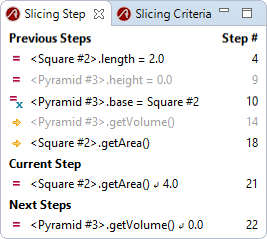
\includegraphics[width=0.80\linewidth]{slice1.png}
	\caption{The Slice Navigator shows context for the current debug step. Steps directly related to the current step are listed in black, steps with overarching dependencies in gray. Small icons indicate how the steps are related.}
	\label{fig:slice1}
\end{figure}

The contributions of this paper are threefold:
\begin{itemize}
	\item The integration of dynamic analyzes directly in the debugger reduces interruptions in developer flow by minimizing context switches between tools and shortens waiting time as recorded run-time data can be re-used.
	\item A new dynamic slicing algorithm allows quick and iterative refinement of the slicing criteria to adapt the slice to changing developer questions.
		Based on previous work, developers can formulate their question by choosing from different dependency types that will change the outcome of the slice.
	\item The \emph{Slice Navigator} is a UI component that bundles access to the debugger and the slicer.
		It provides context for the current instruction by showing relevant parts of the slice, allows developers to iteratively refine the slicing criteria, and serves as an alternative to breakpoints and stepping.
		\todo{mention the improved debugging workflow}.
		
\end{itemize}

The remainder of this paper is structured as follows:
\Cref{sec:workflow} explains the Slice Navigator user interface and how it allows for an improved debugging workflow.
\Cref{sec:impl} discusses relevant details of the implementation and the slicing algorithm.
\Cref{sec:eval} evaluates the feasibility of our approach.
\Cref{sec:conclusion} concludes.

\section{Related Work}

relevance of debugger\\

backwards debugging\\
omniscient debugging\\

slicing weiser \cite{weiser_programmers_1982} \\
dynamic slicing\\
see soot paper\\

\section{A New Debugging Workflow}
\label{sec:workflow}

Both omniscient debugging (ODB) and (dynamic) slicing changed the way how developers approach fault localization.
In this section, we use a simple example to demonstrate how we integrated existing and new tools to an improved debugging workflow.

\todo{we describe ui, info and control}

\subsection{Getting Started}

Very often, the starting point for a debug session is a reproducible observable program failure, preferably in the form of a failing unit test.
Using an omniscient debugger, developers halt the execution at the failing line of code to observe the program state.
From here, they want to backtrack the erroneous state.
However, they quickly realize that the code contains many other side effects making it hard to follow the state of interest.

Using a pure omniscient debugger, developers would now have to track the relation of states to identify the infection chain. In short, they have to manually create a dynamic dependency graph using only their short-term memory.
 
Using our approach, the developer right-clicks the erroneous state in the debugger's variables view and chooses slicing from the context menu.
This will set the variable or field as a slicing criterion and start the slice computation.

%The initial code analysis can take a few seconds.
%The performance of our prototype implementation is evaluated in \todo{section ?} .
Once the slice is computed, all debugging views (e.g., the trace and the variable view) will show instructions or variables not belonging to the slice only in gray.
Stepping through the execution will skip instructions not belonging to the slice.

We will use a small code example to explain the user interface and internals of the slice navigator. 
\Cref{lst:example} shows two Java classes and a failing JUnit test case.
In our scenario, after noticing a failed test case, the developer chooses to slice on the arguments of the ´assertEquals´ invocation in \linerefn{lst:example}{29}.
Because we are using only a minimal example, the resulting slice contains almost the entire program.
When we tested the Slice Navigator on real open source programs, this step often already removed a lot of code.

Nevertheless, for a complex program the initial slice can still be too large to allow an efficient search for the problem.
In this case, the developer can now use the slice navigator to get an overview of the execution and to iteratively adjust the slicing criteria.

\begin{lstlisting}[float=t,label=lst:example,caption={Example program with a failing test case}]
	class Square implements Shape2D {
		private double length;
		public Square(double length) { this.length = length; }
		
		@Override
		public double getArea() { 
			return length * length;
		}
	}
	
	class Pyramid implements Shape3D {
		private Shape2D base;
		private double height;
		public Pyramid(Shape2D baseShape, double height) {
			base = baseShape;
			height = height;
		}
		
		@Override
		public double getVolume() { 
			return base.getArea() * height / 3; 
		}
	}
	
	class PyramidTest {
		@Test
		public void test_getVolume() {
			Shape3D shape = new Pyramid(new Square(2), 6);
			assertEquals(8, shape.getVolume());
		}
	}
\end{lstlisting}

\subsection{The Slice Navigator}

The first purpose of the slice navigator is to aid the developer's short-term memory.
It provides a quick overview over previous and upcoming events, and how they relate to the current instruction.
\Cref{fig:slice1} shows a screenshot of the slice navigator with the execution of the example test-case halted on the ´return´ instruction of ´getArea()´ in \linerefn{lst:example}{7}.

A step, or event, is any instruction that has a side effect on the program state.
"Previous Steps" lists all past events that the curent or future events depend on.
Likewise, "Next Steps" shows all events that depend on the current or previous events.

If a step is shown in black, it has a direct dependency link to the current step.
Steps shown in gray have dependencies that go beyond the current step.
I.e., gray "previous steps" have dependency links to "next steps", and vice versa.

Simply by looking at the previous and next steps, the developer can understand at a glace how the current instruction fits into the greater scheme.
This is particularly useful if the current instruction was reached via a breakpoint, in which case it is not always obvious at which point in time it was hit.

To obtain this kind of information with a regular debugger, developers need to analyze the execution stack and maybe even inspect lower stack frames.
But even then it is not always obvious which of the state that is still reachable is actually used again.
Unlike a typical debugger's variable view, the Slice Navigator only shows relevant variables, and also shows relevant object fields on the first level.

Further, the slice navigator shows details about the dependency graph that was used to compute the current slice.
Small icons indicate how the events of the slice are related.
The meaning of these symbols will be explained in the next subsection.

Debugging with the Slice Navigator is simple:
To investigate the origin of a value, developers can simply click on it to move the execution to that point in time.
This way, the slice navigator allows to efficiently follow infection chains of erroneous state.
Likewise, it is easy to follow up on the impact of an instruction by navigating to its future dependencies.

However, using the Slice Navigator developers can not only control the debugger, they can also adjust the slicing criteria.

\subsection{Interactive Slice Configuration}

The slicing component is based on previous work \todo{[xxx]}.
When building the dependency graph between instructions, the algorithm distinguishes between three types of dependencies.

\emph{Value dependencies} occur when the the value of an instruction is derived from another instruction's value.
In the slice navigator, they are represented with a red equality sign.

Instructions that determine if another instruction can be reached are \emph{reachability dependencies}, indicated by a yellow arrow.
Typically, these are method invocations and instruction in conditional statements.
Sometimes, a value depends on only one of multiple candidate values. 

A \emph{control dependency} determines which of these candidates is used.
More formally, control dependencies are reachability dependencies of value candidates that are not also reachability dependencies of all other candidates.
In the navigator, they are indicated by a blue "X".

Developers can now combine these different dependency types to adjust the slice for specific purposes.
Clicking on an event's dependency symbol brings up a dialog that allows to choose which dependencies of that event to include.
This way developers can, for instance, put a focus on how a value was computed or how an instruction was reached.
It is also possible to remove all dependencies of an event, for instance if it is known to be correct and its history is not of interest, thereby moving the focus of the slice to less well-understood parts of the program.

\begin{figure}
	\centering
		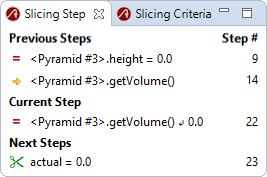
\includegraphics[width=0.80\linewidth]{slice2.png}
	\caption{The program halted at \linerefn{lst:example}{21}, after \lstinline{getArea()} was removed from the slice.}
	\label{fig:slice2}
\end{figure}

Whenever a slicing criterion is modified, the slice is updated instantly, without locking the user interface or resetting the current debug session.
In our examples, developers might choose to exclude the result of ´getArea()´ from the slice as it is correct.
As shown in \cref{fig:slice2}, with the computation of the area removed from the slice it is now much easier to see that the wrong result of ´getVolume()´ was caused by a wrong value in ´height´.

As mentioned before, instructions and states not belonging to the slice are still shown in the IDE, mostly to serve as an orientation help, to provide context to the current operations.
However, it might also happen that a value or instruction outside of the slice catches a developers attention.
In this case, they can choose to add it as another slicing criterion and the slice is immediately expanded.
Again, this happens without interrupting the developer's work.

\todo{move this to evaluation}
%In the worst case, expanding the slice takes as long as creating a new slice for only that event.
%The developer might notice how new events are added to the slice in the background.
%Generally, this should not be an impediment, as events that are closest to the current instruction are added first.

\section{Implementation}
\label{sec:impl}

The Slice Navigator is part of a set of debugging tools that we implemented as a plug-in for the Eclipse IDE.

\subsection{Framework}

The high-level architecture of our prototype consists of three components: the tracer, the event database, and the omniscient debugger including the slicing module.

The tracer is implemented as a Java agent that modifies the bytecode of a program to insert tracing instructions that log all events into csv files.
With our Eclipse plug-in, the developer can initiate an omniscient debug session by selecting a customized launcher in the run configuration.
The launcher will add VM arguments to the execution to configure the tracer.
Once the execution completes, the launcher will automatically import the trace data into a previously configured database.
We provide launchers for basic Java applications and for JUnit test suites.
For JUnit launches, the tracer will treat each test case as an independent execution and ignore code of the testing framework.

The database stores all events of a set of executions.
It is possible to set up one database per project or one for the entire workspace.
We currently support HSQLDB, MySql, and SAP Hana, but in principle any relational database can be used.

The omniscient debugger consists of a set of views that allow to debug a Java application based on the data from the database.
It is a post-mortem debugger, i.e., it simulates a debug session while the actual program has already terminated.

\subsection{Initial slice computation}

\todo{The slicing component is based on previous work [xxx].}
The basic structure is of the algorithm for building the initial slice is fairly simple and shown in \cref{lst:slicealgo}.

\begin{lstlisting}[float=t,language=algorithm,label=lst:slicealgo,caption={Simplified algorithm for building the slice}]
	function build_slice(criteria)
		slice := {}
		for each event \in criteria do ''in parallel''
			add_to_slice(slice, event)
		return slice
		
	function add_to_slice(slice, event)
	  if event \in slice || event.is_negative_criterion then return
		slice += event
		static_dependency_graph := event.method.dependency_graph
		static_dependencies := static_dependency_graph.get( event.instruction, event.dependency_flags)
		for each instruction \in static_dependencies do ''in parallel''
			prev_event := find_last_previous_event(instruction)
			if prev_event ''exists'' then
			  prev_event.inherit_dependency_flags(event)
				add_to_slice(slice, prev_event)
\end{lstlisting}

%\begin{lstlisting}[numberfirstline=true,language=algorithm,firstnumber=1,label=lst:slicealgo,caption={Example program with a failing test case}]
	%function build_slice(criteria)
		%slice := {}
		%for each event \in criteria do ''in parallel''
			%add_to_slice(slice, event)
		%return slice
		%
	%function add_to_slice(slice, event)
		%'add event to slice'
		%'get static dependency graph of event\'s method'
		%'get static dependencies of event\'s instruction'
		%for each instruction \in 'static dependencies' do ''in parallel''
			%'find last previous event at instruction'
			%if 'previous event exists' && 'previous event' \notin slice then
				%add_to_slice(slice, 'previous event')
%\end{lstlisting}

%A static code analysis built with the Soot framework creates static dependency graphs on the method level.
%Static dependency graphs are computed on demand and cached for reuse.

The slicing criterion is a set of events, the slice is initially an empty set.
For each event that is added to the slice, the static dependency graph of the event's method is obtained.

If the graph is not initialized yet, it will be created by a code analysis using the Soot framework \todo{cite}.
The dependency graph contains every instruction's static dependencies and distinguishes between three dependency types, as described in the previous section.
Dependency instruction candidates are looked up in the graph by the event's instruction.

For each candidate instruction, the latest occurrence is looked up in the event database.
For variable assignments the look up is limited to the current method invocation, for events like field assignments the scope is not limited.
If an event was found, it will be added to the slice next.

Every event carries flags that indicate which types of its dependencies the slice should include.
If the dependency flags are empty, the event is considered a negative criterion and is removed entirely from the slice (cf.~\linerefn{lst:slicealgo}{8}).
If the dependency flags of an event were not configured directly by the user, they are inherited from the depending events (cf.~\linerefn{lst:slicealgo}{15}).

\subsection{Incremental slicing}

Adding another event to the slicing criteria works similarly to building a new slice, the major difference being that the slice is not initially empty.

When developers want to remove an event from the slice, we need to know when to cascade the removal to its dependencies.
As the dependency graph is acyclic, we can use reference counting for this.
However, we need to independently count the references for each dependency type.
When the counter for one of the dependency types reaches zero, dependencies of that type are unlinked respectively.

Changing the dependency type of an event, e.g., from value to reachability, is a combination of removing and adding an event.

\subsection{Filling the Slice Navigator}


iterate over slice starting at current step \\
events at current step always collected \\
if one of dependencies was before current step, event is collected as "next steps" \\
dependencies before current collected at "previous steps" \\
events with direct connection to current step are flagged as such

special case: reachability only \\
to prevent entire stack in "previous steps" and entire variable history in "next steps", \\
events are not collected if the only overarching dependency is of reachability type.

second special case: transparent classes\\
classes of the jdk are flagged as transparent\\
all internal events, ie all except direct accesses from non-transparent classes, are resolved immediately and never appear in the navigator.

\section{Evaluation}
\label{sec:eval}

One of the main advantages of the Slice Navigator is that it integrates into the debugging workflow.
As such, it is crucial that results are produced in a timely manner, as a waiting time of even a few seconds may interrupt developers in their flow.

To evaluate the performance of our approach on real-world code, we measured the computation of several slices on JUnit tests of Camunda's open-source BPMN engine\footnote{\todo{link to camunda}}.
All tests were run on a 2.0 GHz Intel i7 Processor with 4 cores and and 8 GB RAM, running Windows 8.1.
A MySql database was used to store the trace data.
We repeated every measurement 10 times, all charts show the average values.

\begin{figure}
	\centering
		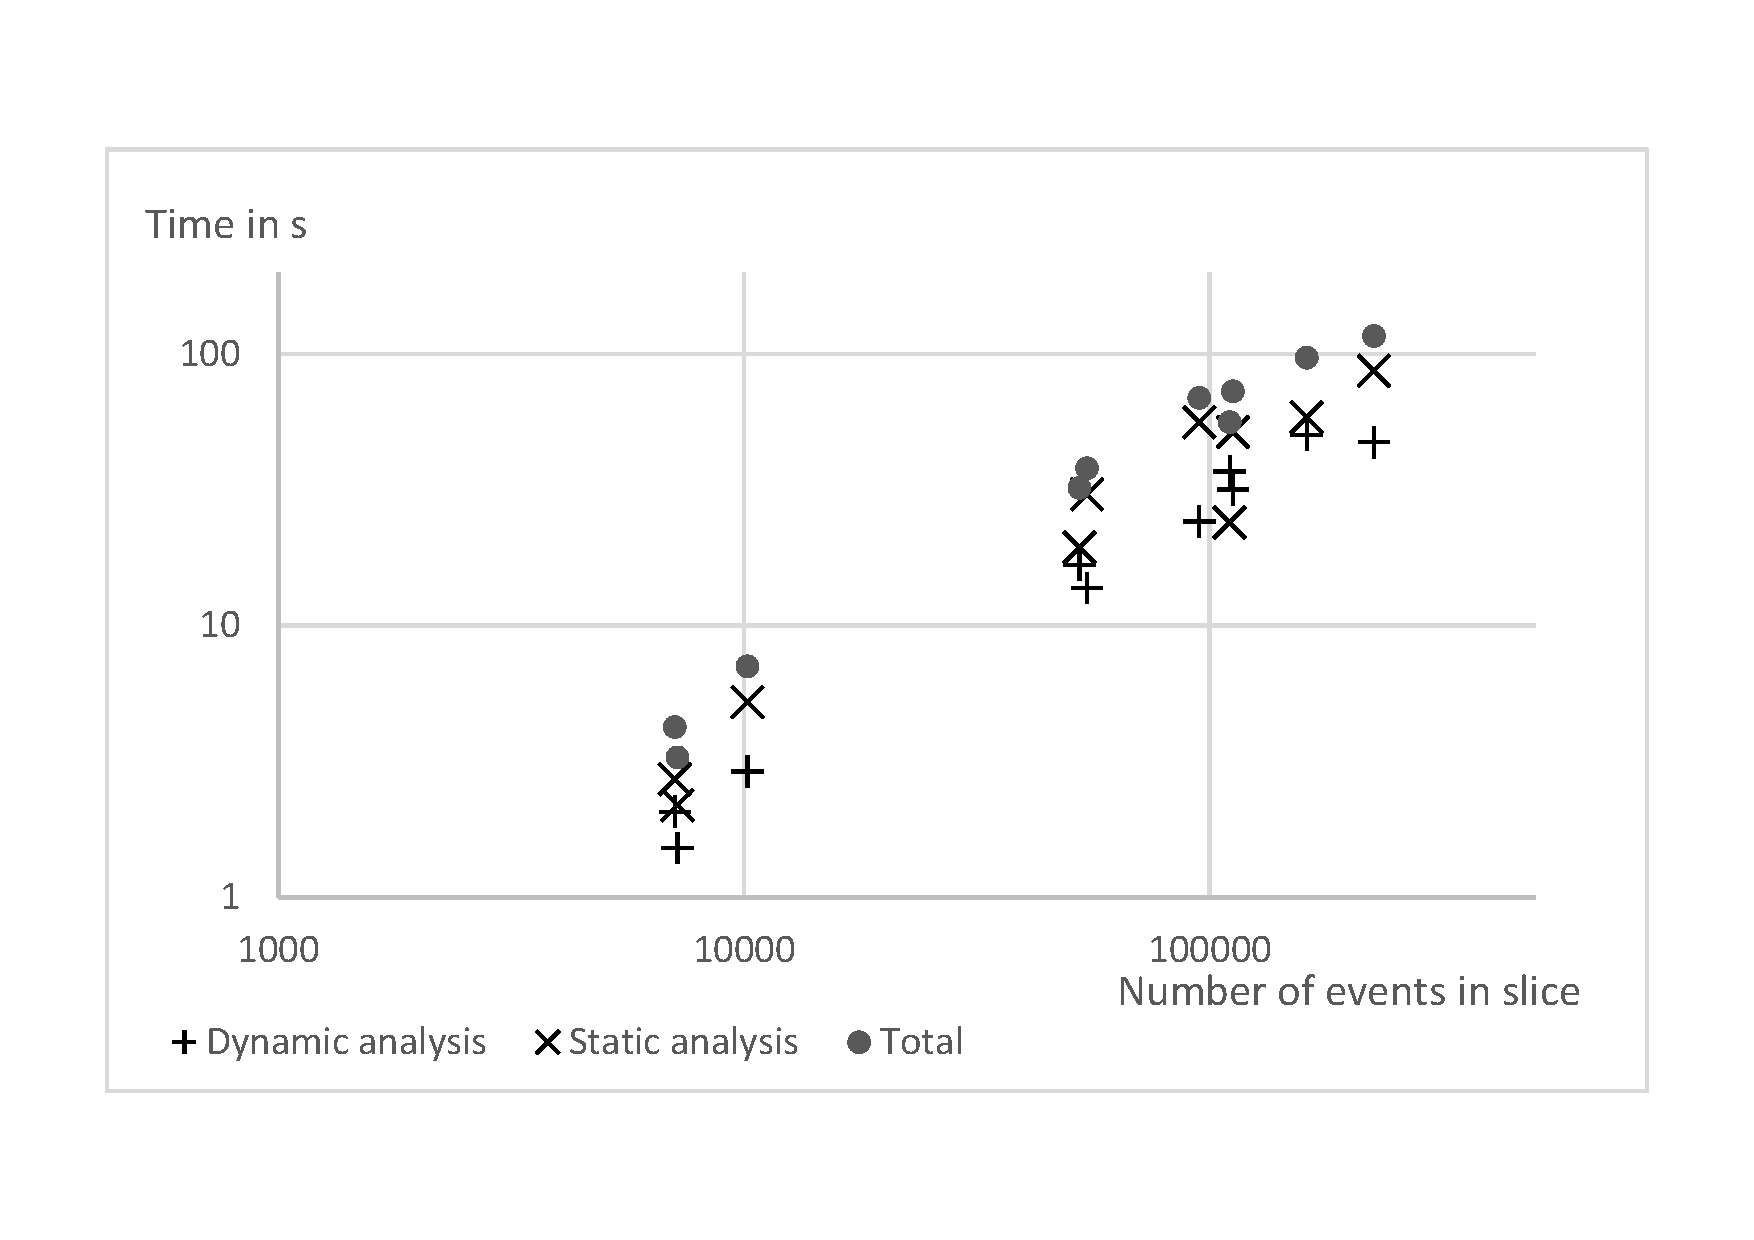
\includegraphics[width=\linewidth, clip, trim={20mm 26mm 20mm 26mm}]{chart-initial.pdf}
	\caption{Time for computing the initial slice}
	\label{fig:chartinitial}
\end{figure}

We previously observed that our approach differs from other slicing implementations insofar as that the run-time of the algorithm does not depend on the total run-time of the sliced program, but only on the size of the resulting slice\todo{cite}.

\Cref{fig:chartinitial} shows the time for computing the initial slice in seconds, depending on size of the resulting slice.
Times are given in total, and divided into static code analysis and the dynamic analysis of the event data.

As can be seen, the static analysis taking slightly more time on average.
It should be noted that the total time is less than the sum of the static and dynamic analysis times, as both can, to some extend, run in parallel.


\begin{figure}
	\centering
		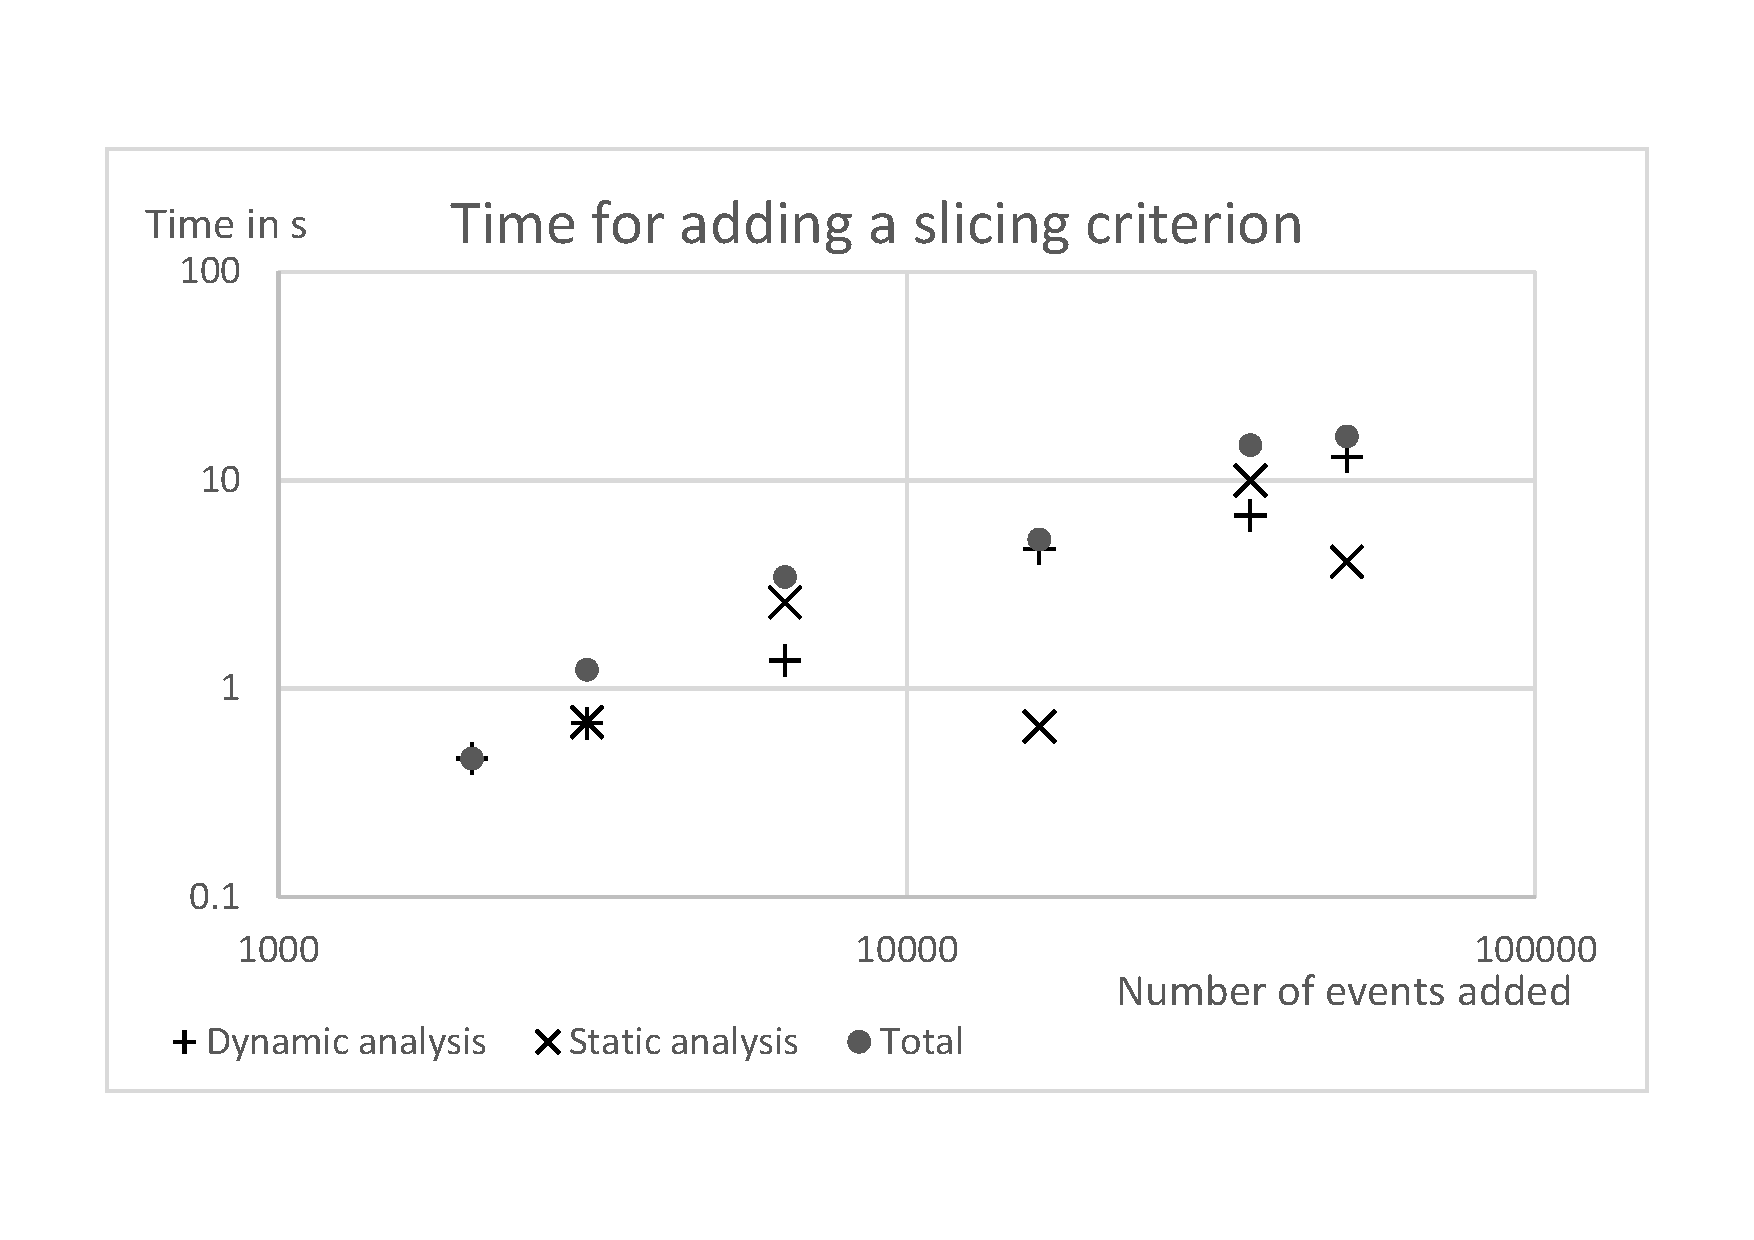
\includegraphics[width=\linewidth, clip, trim={20mm 26mm 20mm 26mm}]{chart-add.pdf}
	\caption{Time for adding a slicing criterion}
	\label{fig:chartadd}
\end{figure}


\begin{figure}
	\centering
		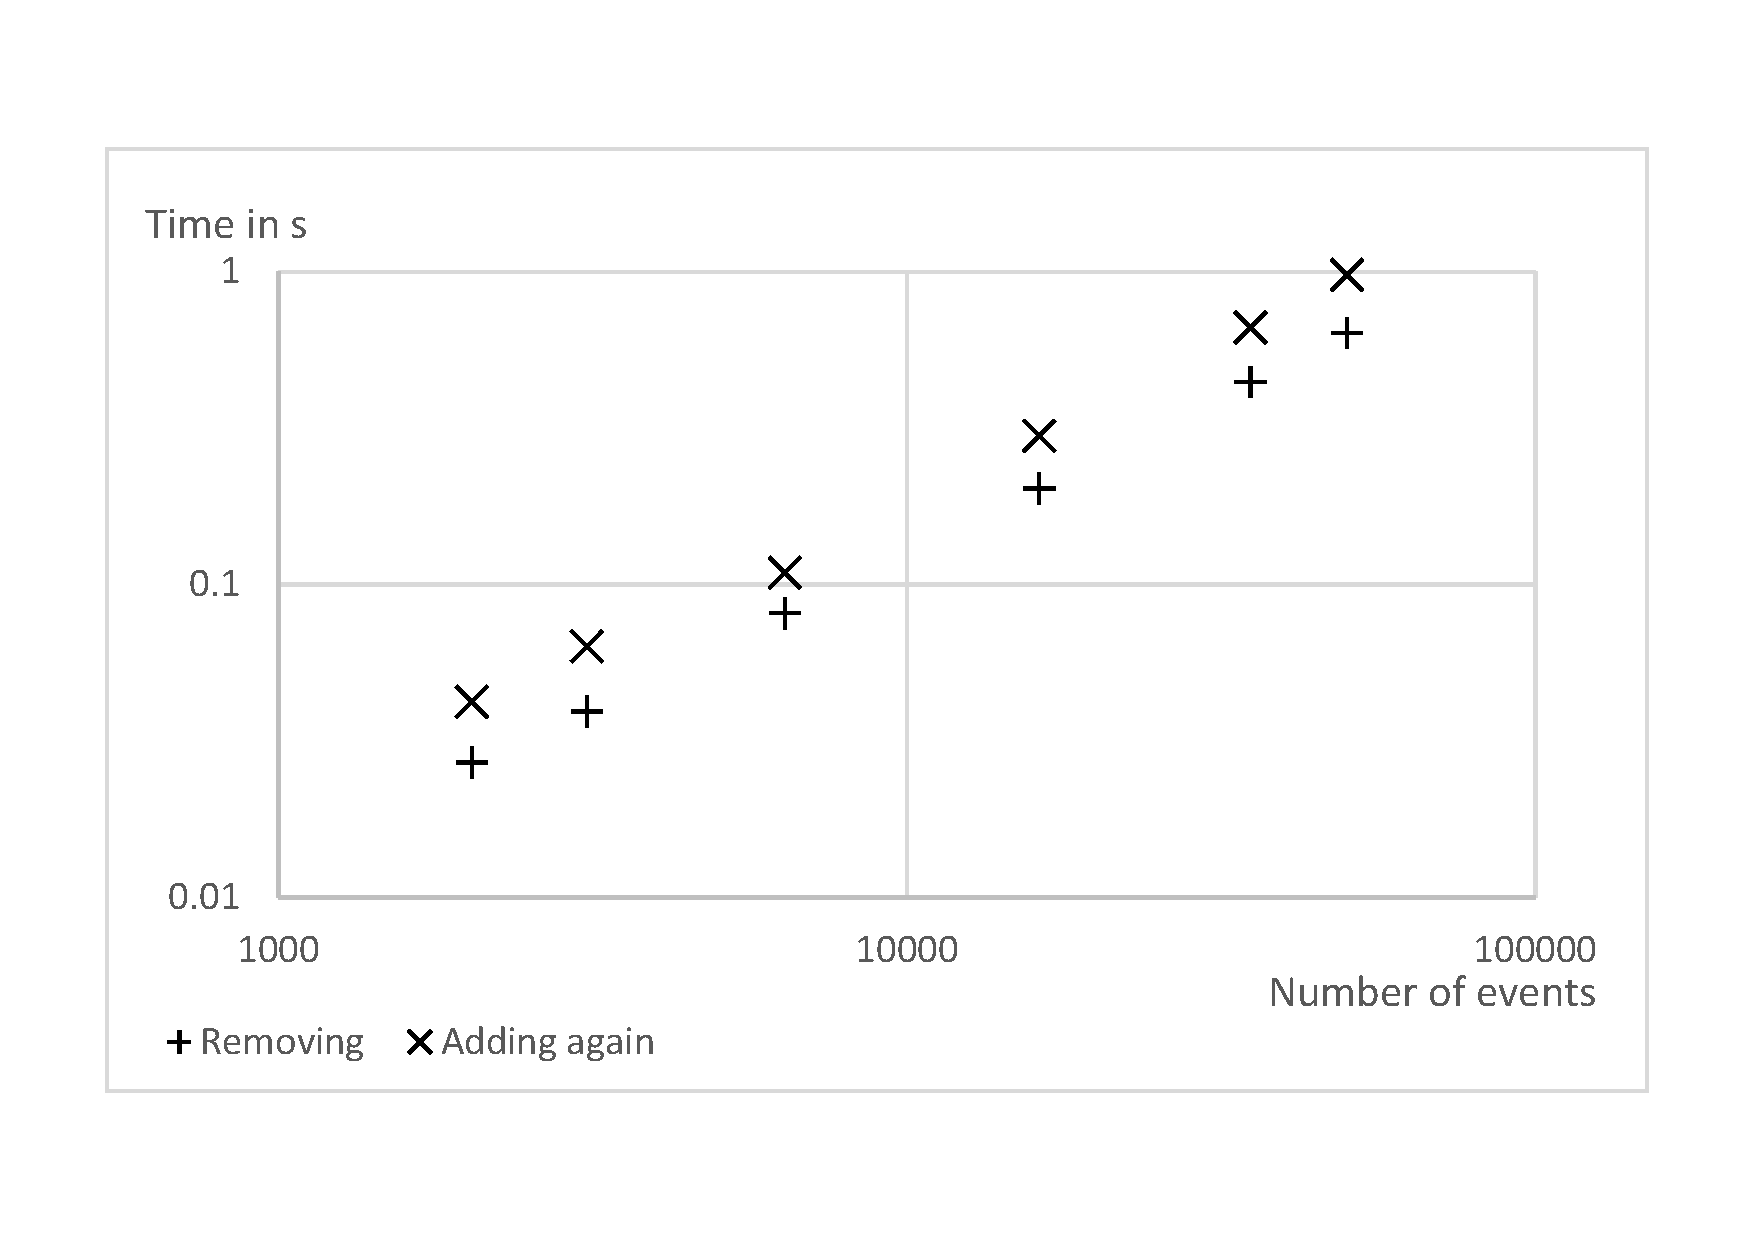
\includegraphics[width=\linewidth, clip, trim={20mm 26mm 20mm 26mm}]{chart-rem.pdf}
	\caption{Time for computing the initial slice}
	\label{fig:chartinitial}
\end{figure}



\section{Conclusion}
\label{sec:conclusion}


\printbibliography

\end{document}